\documentclass{iaii_pai}

% === Additional packages not in cls ===
\usepackage{amsmath,amsfonts}
\usepackage{algorithm}
\usepackage{algpseudocode}
\usepackage{enumitem}
\usepackage{tikz}
\usepackage{adjustbox}
\usepackage[percent]{overpic}

% === Convenience Macros ===
\newcommand{\figref}[1]{\cref{#1}}
\newcommand{\tabref}[1]{\cref{#1}}
\newcommand{\eqnref}[1]{\cref{#1}}
\newcommand{\secref}[1]{\cref{#1}}

% === Paper-Specific Macros ===
\newcommand{\methodname}{PAIWorld}
\newcommand{\loss}{\mathcal{L}}
\newcommand{\lossrepa}{\mathcal{L}_{\text{REPA}}}
\newcommand{\lossdiff}{\mathcal{L}_{\text{diff}}}
\newcommand{\losstotal}{\mathcal{L}_{\text{total}}}
\newcommand{\R}{\mathbb{R}}
\newcommand{\E}{\mathbb{E}}
\newcommand{\feat}{\mathbf{z}}
\newcommand{\featthree}{\mathbf{f}_{\text{3D}}}
\newcommand{\proj}{\mathbf{P}}
\newcommand{\pose}{\boldsymbol{\pi}}
\newcommand{\argmin}{\operatorname{argmin}}

% === Graphics Path ===
\graphicspath{{figures/}}

% === Title ===
\title{PAIWorld: A 3D-Consistent Multi-View World Foundation Model for Robotic Manipulation}

% === Authors ===
\author[1]{The PAI Lab}

% === Affiliations ===
\affiliation[1]{Institute of AI for Industries, Chinese Academy of Sciences}

% === Metadata ===
\date{June 2026}

% === Abstract ===
\abstract{%
World foundation models (WFMs) have emerged as powerful simulators of physical environments, yet they predominantly operate in a single-view setting and lack the multi-view 3D consistency that robotic manipulation demands. Robotic systems inherently rely on multiple cameras---egocentric, eye-to-hand, and wrist-mounted---to capture complementary viewpoints for policy learning. Current multi-view world models, however, simply concatenate view tokens without explicit geometric reasoning, yielding cross-view object drift, depth inconsistency, and texture misalignment that propagate errors into downstream planning and control. We trace these failures to two fundamental deficiencies: (1)~the absence of an explicit \emph{inter-view communication mechanism}, which forces each viewpoint to generate in isolation, and (2)~the absence of a \emph{3D geometric prior}, which leaves the model without guidance on what constitutes physically correct cross-view structure. We argue that resolving both is necessary and sufficient: an information pathway across views and a geometric signal that steers it must coexist, since communication without geometric guidance collapses to trivial shortcuts, while geometric priors without an inter-view channel cannot propagate constraints across viewpoints. Building on this analysis, we present \methodname{}, a framework that augments diffusion-transformer world models with three components: \textbf{Geometric Rotary Position Embedding} encodes camera ray directions and extrinsic poses into the attention mechanism via rotary position encoding; \textbf{Geometry-Aware Cross-View Attention} blocks provide explicit inter-view communication channels; and \textbf{Latent 3D-REPA} distills 3D-aware features from frozen 3D foundation models as the geometric learning signal. Built upon the Cosmos world foundation model, \methodname{} attains state-of-the-art multi-view 3D consistency on robotic manipulation benchmarks and enables downstream applications including model-based planning, world action models, and multi-view policy post-training.%
}

\begin{document}

\maketitle

\section{Introduction}
\label{sec:introduction}

World foundation models (WFMs) have rapidly progressed from compact latent-dynamics modules~\cite{ha2018world,hafner2020dreamer} to large-scale video generation systems capable of simulating complex physical environments~\cite{nvidia2025cosmos,liu2024sora,yang2024cogvideox,gao2024vista}. By learning to predict future visual observations conditioned on actions or text, WFMs serve as \emph{world simulators} that can be leveraged for model-based planning~\cite{wu2023daydreamer}, policy evolution~\cite{du2024learning}, and data synthesis in robotic learning~\cite{zhou2024robodreamer}. The Cosmos platform~\cite{nvidia2025cosmos}, in particular, has demonstrated that diffusion-transformer (DiT) architectures~\cite{peebles2023dit} trained on internet-scale video data can produce temporally coherent, physically plausible visual rollouts, making WFMs a promising backbone for embodied intelligence.

However, robotic manipulation systems are inherently \emph{multi-view} systems. Standard configurations employ wrist-mounted and egocentric cameras simultaneously to provide complementary geometric and semantic information for policy learning~\cite{brohan2023rt1,brohan2023rt2,collaboration2023openx}. When a world model is deployed as a simulated generator for such systems, it must generate future observations across all viewpoints while maintaining strict 3D consistency: the same object must appear at geometrically compatible locations, with coherent depth and texture, across all views at every time step. Failure to maintain this consistency--manifesting as cross-view object drift, depth contradictions, or texture misalignment--directly undermines the physical plausibility of imagined trajectories and propagates errors to downstream planning and control~\cite{wu2023daydreamer,chi2023diffusionpolicy}.

Existing approaches to multi-view world modeling fall short of this requirement. Single-view WFMs such as Cosmos~\cite{nvidia2025cosmos}, CogVideoX~\cite{yang2024cogvideox}, and Vista~\cite{gao2024vista} produce high-quality temporal predictions but are architecturally restricted to one viewpoint. Methods that do handle multiple views, such as Genie~\cite{bruce2024genie} and iVideoGPT~\cite{wu2024ivideogpt}, typically concatenate tokens from different viewpoints along the sequence dimension without introducing explicit mechanisms for cross-view geometric reasoning. This ``flat concatenation'' strategy treats multi-view tokens identically to temporal tokens, leaving the model to discover cross-view correspondences implicitly from data. This implicit discovery becomes increasingly unreliable as the number of viewpoints and the complexity of the scene grow.

We trace the root cause of these failures to two fundamental deficiencies in existing multi-view approaches. First, they lack an explicit \emph{inter-view communication mechanism}. The flat concatenation strategy provides no dedicated pathway for viewpoints to exchange information; each view's tokens attend to the entire sequence without distinguishing same-view from cross-view tokens, forcing the model to discover geometric correspondences implicitly from data. As a result, each viewpoint effectively generates in isolation, with no way to coordinate predictions or resolve cross-view conflicts. Second, they lack a \emph{3D geometric prior}. Even with an inter-view communication pathway, the model has no supervision signal specifying what geometrically consistent 3D structure looks like. Without explicit geometric guidance, cross-view information exchange tends to converge on superficial shortcuts, such as matching color palettes or copying textures, rather than learning true 3D correspondences.

These two deficiencies demand two corresponding solutions: an information pathway that enables cross-view coordination, and a geometric learning signal that steers this pathway toward 3D-correct representations. Importantly, \emph{neither solution alone is sufficient}. An inter-view communication channel (Cross-View Attention) without geometric guidance allows information to flow across views but provides no guarantee that the exchanged information respects 3D geometry. In practice it learns shortcuts such as texture copying or uniform averaging. Conversely, a 3D geometric prior (Latent 3D-REPA, which aligns DiT representations with features from frozen 3D foundation models~\cite{wang2025vggt,lin2025depthanything3}) improves each view's 3D awareness independently, but without an inter-view channel, the geometric constraints cannot propagate across viewpoints and cross-view inconsistencies persist. Only when both are present does the system achieve genuine multi-view 3D consistency: the communication channel carries geometrically meaningful content, and the geometric prior is enforced coherently across all views.

Based on this analysis, we present \textbf{\methodname{}}, a framework that augments the Cosmos DiT backbone with three lightweight, modular components designed to jointly satisfy both conditions (\figref{fig:pipeline}). A shared \emph{Geometric Rotary Position Embedding} (Geo-RoPE) encodes camera ray directions and extrinsic poses into the attention mechanism via rotary position encoding~\cite{su2024rope,he2024cameractrl}, providing the common geometric reference frame. \emph{Cross-View Attention} blocks, interleaved within the DiT, provide the inter-view communication channel. \emph{Latent 3D-REPA} supplies the 3D geometric prior by aligning intermediate DiT features with 3D-aware representations from 3D foundation models via the REPA framework~\cite{yu2024repa}. Our contributions are as follows:
\begin{itemize}
	\item We identify two fundamental deficiencies in existing multi-view world models, namely the lack of inter-view communication and the absence of 3D geometric priors, and show that addressing both simultaneously is necessary and sufficient for multi-view 3D consistency.
	\item We introduce \methodname{}, which satisfies both conditions through Cross-View Attention, Latent 3D-REPA, and Geometric Rotary Position Embedding. These three plug-and-play modules are applicable to any DiT-based world model.
	\item We demonstrate that \methodname{} achieves state-of-the-art multi-view 3D consistency on robotic manipulation benchmarks, and that the improved consistency directly benefits downstream embodied tasks including model-based robotic planning and world action model fine-tuning.
\end{itemize}

The remainder of this paper is organized as follows. \secref{sec:related-work} reviews related work on world models, multi-view generation, and 3D-aware representations. \secref{sec:methods} presents the \methodname{} framework in detail. \secref{sec:conclusion} summarizes our findings and discusses future directions.

\section{Related Work}
\label{sec:related-work}

\subsection{World Foundation Models for Physical AI}

The concept of learning internal models of the environment, commonly known as world models, has a long history in reinforcement learning and cognitive science~\cite{ha2018world}. Early approaches such as Dreamer~\cite{hafner2020dreamer} and DayDreamer~\cite{wu2023daydreamer} learn compact latent-state dynamics models that enable planning through imagined rollouts, demonstrating the viability of model-based learning for physical robot control. More recently, the success of large-scale generative models has motivated a paradigm shift toward \emph{world foundation models} (WFMs) that operate directly in pixel or video space. Sora~\cite{liu2024sora} demonstrated that video diffusion models can generate temporally coherent, physically plausible visual simulations. The Cosmos platform~\cite{nvidia2025cosmos} further formalized this direction by training DiT-based~\cite{peebles2023dit} video generation models on internet-scale data for physical AI applications, while Cosmos 3~\cite{nvidia2026cosmos3} extended it to an omnimodal framework unifying language, image, video, audio, and action modalities. CogVideoX~\cite{yang2024cogvideox}, HunyuanVideo~\cite{kong2024hunyuanvideo}, Stable Video Diffusion~\cite{blattmann2023svd}, and Wan~\cite{wan2025wan} achieved high-fidelity video generation across diverse domains. DIAMOND~\cite{alonso2024diamond} demonstrated that diffusion-based world models can capture fine visual details critical for decision-making. Pelican-Unified~\cite{zhang2026pelican} advocates a unified paradigm integrating world modeling with understanding, reasoning, and action for embodied intelligence. However, these models are fundamentally single-view: they generate one coherent video stream without explicit mechanisms for multi-view consistency.

Interactive world models represent another important direction. UniSim~\cite{yang2023unisim} learns real-world simulators from diverse data sources, Genie~\cite{bruce2024genie} and Genie 2~\cite{parkerholder2024genie2} enable interactive environment generation from single images, and iVideoGPT~\cite{wu2024ivideogpt} scales autoregressive world models to complex environments. In the robotic manipulation domain, GR-2~\cite{cheang2024gr2} builds a generative video-language-action model with web-scale knowledge, IRASim~\cite{zhu2025irasim} learns action-conditioned video simulators from real robot data, EnerVerse~\cite{huang2025enerverse} envisions embodied future spaces for manipulation planning, and LaDi-WM~\cite{huang2025ladiwm} employs latent diffusion-based world models for predictive manipulation. AgiBot World~\cite{bu2025agibotworld} provides a large-scale multi-view manipulation platform, and WorldArena~\cite{shang2026worldarena} offers a unified benchmark for evaluating embodied world models. While some of these systems support multiple viewpoints via token concatenation, none introduces explicit cross-view geometric reasoning---a critical limitation for robotic applications, where 3D consistency directly governs policy quality.

\subsection{Multi-View and 3D-Aware Visual Generation}

Multi-view generation has been extensively studied in the context of 3D content creation from single images. Zero-1-to-3~\cite{liu2023zero123} pioneered viewpoint-conditioned diffusion by fine-tuning a 2D diffusion model with relative camera transformations. SyncDreamer~\cite{liu2023syncdreamer} introduced synchronized multi-view denoising with 3D-aware attention to ensure geometric consistency across generated views. MVDream~\cite{shi2023mvdream} extended multi-view diffusion to text-conditioned 3D generation, while MVDiffusion~\cite{tang2023mvdiffusion} enabled holistic multi-view image generation with correspondence-aware attention. SV3D~\cite{voleti2024sv3d} leveraged latent video diffusion for orbital multi-view synthesis, and SV4D~\cite{xie2024sv4d} further extended this to dynamic 3D content with multi-frame and multi-view consistency. CAT3D~\cite{gao2024cat3d} demonstrated that multi-view diffusion models can create high-quality 3D assets from arbitrary inputs. These methods demonstrate that explicit view-conditioning and cross-view interaction mechanisms can produce 3D-consistent multi-view images. However, they are designed for \emph{static} or short-sequence object-centric scenes and do not address generating consistent multi-view \emph{videos} of dynamic environments as required by world models.

Camera control in video generation has been explored by CameraCtrl~\cite{he2024cameractrl}, which represents camera poses using Pl\"ucker ray coordinates and injects them into video diffusion models. ViewCrafter~\cite{yu2024viewcrafter} further tames video diffusion models for high-fidelity novel view synthesis. These works provide technical foundations for camera-aware generation, but focus on single-view camera trajectory control rather than multi-view consistency.

\subsection{3D Representations and Geometric Reconstruction}

Recent advances in geometric 3D vision have produced powerful tools for evaluating and enforcing 3D consistency. Neural Radiance Fields (NeRF)~\cite{mildenhall2020nerf} and 3D Gaussian Splatting~\cite{kerbl2023gaussiansplatting} established the foundation for differentiable 3D scene representations. DUSt3R~\cite{wang2024dust3r} and its successor MASt3R~\cite{leroy2024mast3r} learn to predict dense 3D point maps from image pairs without requiring known camera parameters, enabling direct measurement of cross-view geometric consistency. The Depth Anything series~\cite{yang2024depthanything,yang2024depthanythingv2,lin2025depthanything3} provides foundation models for monocular depth estimation that capture robust 3D-aware features from large-scale training. VGGT~\cite{wang2025vggt} further advances this direction by grounding visual geometry in a unified transformer that jointly predicts camera poses, depth, and 3D point maps from arbitrary image collections. These models encode rich geometric priors that can serve as supervision targets for world models seeking 3D consistency.

The REPA framework~\cite{yu2024repa} introduced the idea of aligning intermediate representations of diffusion transformers with those of pretrained encoders, demonstrating accelerated training and improved generation quality for image diffusion. Our Latent 3D-REPA extends this principle from 2D image generation to multi-view video world models, using 3D-aware features from VGGT and Depth Anything 3 as the alignment target to inject geometric consistency directly into the diffusion process.

% \subsection{Robotic World Models and Embodied AI}

% The application of world models to robotics has gained significant momentum. RoboDreamer~\cite{zhou2024robodreamer} learns compositional world models that enable robot imagination for planning. The Open X-Embodiment initiative~\cite{collaboration2023openx} and associated RT-X models provide large-scale multi-robot datasets and policies, establishing the standard multi-camera configuration (wrist, overhead, egocentric) for robotic manipulation. RT-1~\cite{brohan2023rt1} and RT-2~\cite{brohan2023rt2} demonstrated scalable robotic control via transformers, while BridgeData V2~\cite{walke2023bridgedata} and RoboCasa~\cite{nasiriany2024robocasa} provide diverse manipulation data. Octo~\cite{octo2024} offers a generalist policy trained on multi-embodiment data, and $\pi_0$~\cite{black2024pi0} shows that vision-language-action flow models can achieve general robot control. NVIDIA's GR00T~\cite{nvidia2025groot} further scales foundation models for humanoid robots.

% These works highlight that modern robotic systems fundamentally rely on multi-view observations, yet the world models that serve them remain predominantly single-view. \methodname{} bridges this gap by providing a 3D-consistent multi-view world model backbone that can directly serve as a simulator for multi-camera robotic planning and policy learning.

% \subsection{Diffusion Transformers and Positional Encoding}

% Our work builds upon the Diffusion Transformer (DiT) architecture~\cite{peebles2023dit}, which replaces U-Net backbones with transformer blocks for diffusion-based generation. DiT's flexibility in handling variable-length token sequences makes it naturally suited to multi-view inputs. Rotary Position Embedding (RoPE)~\cite{su2024rope} provides an efficient mechanism for encoding positional information that preserves relative position relationships, a property we exploit in our Geometric Rotary Position Embedding to encode camera geometry directly into the attention mechanism. The latent diffusion paradigm~\cite{rombach2022ldm,ho2020ddpm} operates in a compressed representation space, which both reduces computational cost and provides the natural setting for our latent-level representation alignment.

\section{Method}
\label{sec:methods}

\begin{figure*}[t]
	\centering
	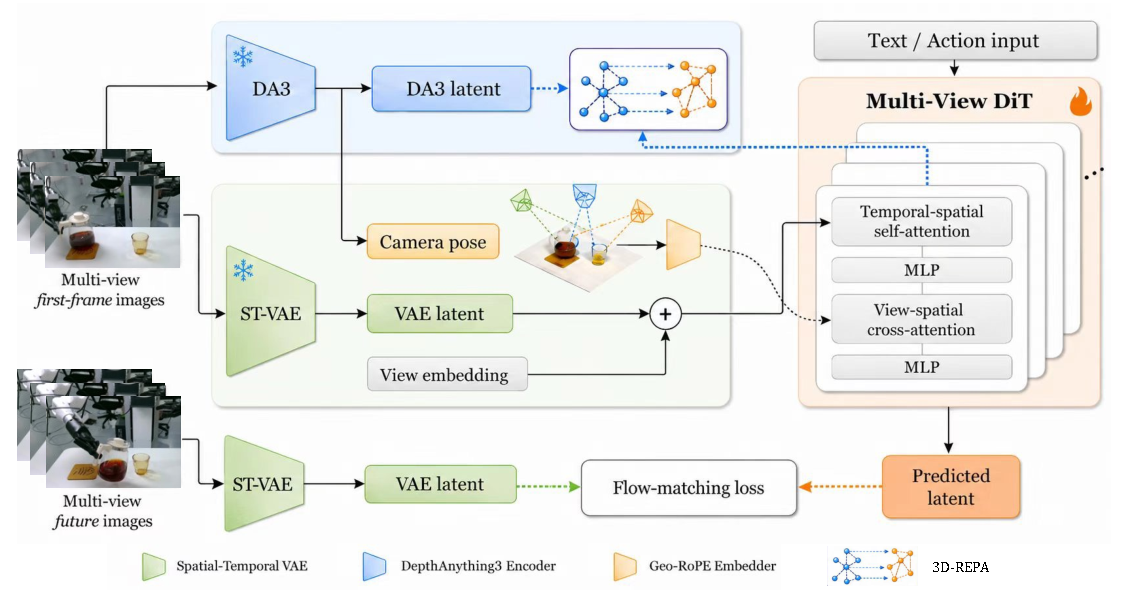
\includegraphics[width=\textwidth]{pipeline.pdf}
	\caption{Overview of the \methodname{} framework. Built upon a DiT-based flow matching backbone, \methodname{} introduces three components to achieve multi-view 3D consistency: (1)~Geometric Rotary Position Embedding (Geo-RoPE) encodes camera ray directions and extrinsic poses into the attention mechanism, (2)~Cross-View Attention blocks enable explicit inter-view communication, and (3)~Latent 3D-REPA aligns intermediate DiT representations with 3D-aware features from frozen foundation models (VGGT). The three components jointly satisfy the two necessary conditions for multi-view 3D consistency: inter-view communication and 3D geometric priors.}
	\label{fig:pipeline}
\end{figure*}

We present \methodname{}, a framework for injecting 3D consistency into flow-matching-based world foundation models for multi-view robotic manipulation. As analyzed in \secref{sec:introduction}, multi-view 3D consistency requires two conditions: inter-view communication and 3D geometric priors. Our approach augments a DiT-based flow matching backbone with three components that jointly satisfy both conditions (see \figref{fig:pipeline}): Geometric Rotary Position Embedding (\secref{sec:camera-pe}), Cross-View Attention (\secref{sec:cross-view-attn}), and Latent 3D-REPA (\secref{sec:3d-repa}). We first formalize the problem setting (\secref{sec:problem}), then describe each component and analyze why both conditions must be satisfied simultaneously (\secref{sec:synergy}).

\subsection{Problem Formulation}
\label{sec:problem}

Consider a robotic manipulation system equipped with $V$ cameras, each providing a video stream. At time step $t$, the system observes a set of images $\{I_t^v\}_{v=1}^{V}$ with associated camera intrinsics $\{\mathbf{K}^v\}_{v=1}^{V}$ and extrinsics $\{[\mathbf{R}^v \mid \mathbf{t}^v]\}_{v=1}^{V} \in \mathrm{SE}(3)$. Given a conditioning signal $c$ (text description or action sequence) and a set of context frames, a multi-view world model generates future observations $\{I_{t_0+1:T}^{1:V}\}$ across all viewpoints simultaneously.

The key requirement is \emph{multi-view 3D consistency}: for any 3D point $\mathbf{X} \in \R^3$ visible in views $v_i$ and $v_j$ at time $t$, its projected 2D locations must satisfy the epipolar constraint induced by the relative camera pose. More broadly, the generated multi-view video should admit a coherent 3D reconstruction at every time step.

\subsection{Baseline: Flow Matching DiT for Video Generation}

We adopt a Diffusion Transformer (DiT)~\cite{peebles2023dit} trained with a flow matching objective operating in the latent space of a pretrained video VAE. Given an input video, the VAE encoder produces a latent representation $\feat_0 \in \R^{T \times H \times W \times C}$. The model learns a velocity field $v_\theta(\feat_s, s)$ that transports samples from a noise distribution toward the data distribution along a linear interpolation path:
\begin{equation}
\label{eq:flow-matching}
\feat_s = (1 - s) \feat_0 + s \boldsymbol{\epsilon}, \quad \boldsymbol{\epsilon} \sim \mathcal{N}(\mathbf{0}, \mathbf{I}),
\end{equation}
where $s \in [0, 1]$ is the flow timestep. The training objective minimizes:
\begin{equation}
\label{eq:flow-loss}
\lossdiff = \E_{s, \boldsymbol{\epsilon}}\left[\|v_\theta(\feat_s, s) - (\boldsymbol{\epsilon} - \feat_0)\|_2^2\right].
\end{equation}

\paragraph{Conditioning Signal Injection.}
The conditioning signal $c$ is injected into each DiT block via Adaptive Layer Normalization (AdaLN)~\cite{peebles2023dit}. For text-conditioned generation, $c$ is a text embedding that modulates the scale and shift parameters of layer normalization, globally steering the generation toward the described scene. For action-conditioned generation, rather than representing robot actions as raw vectors, we follow EVAC~\cite{huang2025evac} and render actions into spatial \emph{action maps} that are concatenated with the noisy latent along the channel dimension. This spatial representation preserves the geometric structure of the action (e.g., end-effector trajectory projected into each camera view), enabling the model to ground action semantics in pixel space rather than learning an implicit mapping from abstract action vectors.

\paragraph{Multi-View Token Concatenation.}
For multi-view generation, a naive approach concatenates all view tokens along the sequence dimension, yielding $\feat_0^{\text{concat}} \in \R^{(V \cdot T) \times H \times W \times C}$. While the standard temporal self-attention operates over this concatenated sequence, it treats multi-view tokens identically to temporal tokens without any geometric inductive bias. The model must discover cross-view correspondences entirely from data, which is insufficient for consistent 3D generation.

\subsection{Geometric Rotary Position Embedding}
\label{sec:camera-pe}

To encode 3D geometric information into the attention mechanism, we introduce a \emph{Geometric Rotary Position Embedding} (Geo-RoPE) that separately encodes pixel-level ray directions and view-level camera poses via rotary position encoding~\cite{su2024rope}.

\paragraph{Dual-Component Design.}
For each attention head with dimension $d$, we split the query and key vectors into two equal subspaces: a \emph{ray subspace} of dimension $d_r = d/2$ and a \emph{pose subspace} of dimension $d_p = d/2$. Each subspace receives its own geometric encoding via RoPE.

\paragraph{Ray Component.}
For each token at spatial location $(h, w)$ in view $v$, we compute the world-space ray direction by unprojecting the pixel through the camera intrinsics $\mathbf{K}^v$ and rotating by the inverse of the camera rotation $(\mathbf{R}^v)^{-1}$:
\begin{equation}
\label{eq:ray-dir}
\mathbf{d}^v(h,w) = \text{normalize}\left((\mathbf{R}^v)^\top \cdot (\mathbf{K}^v)^{-1} \begin{pmatrix} h + 0.5 \\ w + 0.5 \\ 1 \end{pmatrix}\right) \in \R^3.
\end{equation}
The 3D ray direction is cyclically expanded to fill the $d_r/2$ frequency slots and used as position coordinates for RoPE rotation on the ray subspace of $\mathbf{q}$ and $\mathbf{k}$.

\paragraph{Pose Component.}
For each view $v$, we extract a 12-dimensional pose feature vector that captures the full camera geometry:
\begin{equation}
\label{eq:pose-feat}
\mathbf{e}^v = [\underbrace{\text{yaw}, \text{pitch}, \text{roll}}_{\text{Euler angles}},\; \underbrace{\mathbf{t}^v}_{\text{translation}},\; \underbrace{-(\mathbf{R}^v)^\top \mathbf{t}^v}_{\text{camera position}},\; \underbrace{(\mathbf{R}^v)^\top \mathbf{e}_z}_{\text{optical axis}}] \in \R^{12},
\end{equation}
where $\mathbf{e}_z = [0,0,1]^\top$. This pose vector is shared across all spatial positions within a view and applied via RoPE to the pose subspace.

\paragraph{Split-RoPE Application.}
The complete Geo-RoPE operates as:
\begin{equation}
\label{eq:geo-rope}
\begin{aligned}
\mathbf{q}_{\text{ray}},\, \mathbf{q}_{\text{pose}} &= \text{split}(\mathbf{q},\; [d_r, d_p]) \\
\tilde{\mathbf{q}}_{\text{ray}} &= \text{RoPE}(\mathbf{q}_{\text{ray}},\; \mathbf{d}^v(h,w)) \\
\tilde{\mathbf{q}}_{\text{pose}} &= \text{RoPE}(\mathbf{q}_{\text{pose}},\; \mathbf{e}^v) \\
\tilde{\mathbf{q}} &= [\tilde{\mathbf{q}}_{\text{ray}};\; \tilde{\mathbf{q}}_{\text{pose}}]
\end{aligned}
\end{equation}
The same operation applies to keys. This design ensures that the ray subspace captures fine-grained pixel-level geometric correspondences (tokens viewing the same 3D point receive similar rotations), while the pose subspace encodes view-level identity (tokens from the same camera share identical pose rotations). Separating the two prevents interference between the spatially-varying ray signal and the spatially-uniform pose signal.

\subsection{Cross-View Attention (Inter-View Communication)}
\label{sec:cross-view-attn}

Standard temporal self-attention in each DiT block operates independently per view (after merging $V$ into the batch dimension), providing no explicit cross-view interaction. We introduce two complementary mechanisms for inter-view communication.

\paragraph{Multi-View Self-Attention Blocks.}
At selected layers (the first 3 and last 3 blocks of the DiT), we insert a dedicated \emph{Cross-View Attention} sub-block. For each time step $t$, let $\{\mathbf{Z}_t^v\}_{v=1}^{V}$ denote the feature maps from all views, where $\mathbf{Z}_t^v \in \R^{(H \cdot W) \times D}$. The Cross-View Attention computes:
\begin{equation}
\label{eq:cross-view-attn}
\hat{\mathbf{Z}}_t^v = \mathbf{Z}_t^v + \text{gate} \cdot \text{Attn}\!\left(\underbrace{\mathbf{Z}_t^v}_{\text{query}},\; \underbrace{[\mathbf{Z}_t^1; \ldots; \mathbf{Z}_t^V]}_{\text{key/value}}\right),
\end{equation}
where $[\cdot;\cdot]$ denotes concatenation along the token dimension, and Attn uses Geo-RoPE for query and key projections so that geometrically corresponding tokens across views naturally receive higher attention weights. The gate is initialized to zero via AdaLN-Zero, ensuring the pretrained single-view model is preserved at initialization.

\paragraph{Spatial-Concat Self-Attention.}
Every 4th block, instead of per-view temporal attention, we concatenate the view and spatial dimensions ($V \times H$) and perform joint spatio-view self-attention over all tokens simultaneously. This provides a broader receptive field where each token can attend to all spatial positions across all views within the same temporal context, complementing the dedicated cross-view blocks.

\paragraph{Why Communication Alone Is Insufficient.}
Cross-View Attention provides the information pathway for viewpoints to exchange geometric and semantic information. Without it, each view's features evolve independently during the flow matching process, with no mechanism to enforce cross-view coherence. However, communication alone does not guarantee 3D consistency: without an explicit 3D learning objective, the cross-view attention can converge to trivial solutions such as copying textures across views or learning shortcut correlations that do not respect true 3D geometry.

\subsection{Latent 3D-REPA (3D Geometric Prior)}
\label{sec:3d-repa}

To provide the geometric learning signal for cross-view interaction, we introduce Latent 3D-REPA, a token-relation distillation objective that aligns the DiT's intermediate representations with features from frozen 3D foundation models.

\paragraph{3D-Aware Feature Extraction.}
We employ VGGT~\cite{wang2025vggt} as our 3D-aware feature extractor. For each multi-view frame set $\{I_t^v\}_{v=1}^V$, VGGT produces dense 1536-dimensional features that encode rich geometric priors including depth, 3D point maps, and camera-relative spatial structure. In addition, VGGT provides predicted camera extrinsics and intrinsics that are used by Geo-RoPE and for 3D point map reconstruction.

\paragraph{Token Relation Distillation.}
Rather than directly regressing 3D features token-by-token, we distill the \emph{relational structure} between tokens. At a selected intermediate layer $\ell$ of the DiT (layer 18 in our implementation), we extract the feature map $\mathbf{H}_\ell \in \R^{(T \cdot V \cdot H \cdot W) \times D}$ and project it to the VGGT feature dimension via a lightweight 3D convolutional projector $g_\phi$. The distillation loss operates on pairwise token similarities:
\begin{equation}
\label{eq:3d-repa}
\lossrepa = \alpha \cdot \mathcal{L}_{\text{spatial}} + \beta \cdot \mathcal{L}_{\text{temporal}},
\end{equation}
where the spatial loss enforces intra-frame token relations:
\begin{equation}
\mathcal{L}_{\text{spatial}} = \text{SmoothL1}\!\left(\mathbf{S}^{\text{DiT}}_{\text{intra}},\; \mathbf{S}^{\text{VGGT}}_{\text{intra}}\right),
\end{equation}
and the temporal loss enforces inter-frame token relations:
\begin{equation}
\mathcal{L}_{\text{temporal}} = \text{SmoothL1}\!\left(\mathbf{S}^{\text{DiT}}_{\text{inter}},\; \mathbf{S}^{\text{VGGT}}_{\text{inter}}\right).
\end{equation}
Here $\mathbf{S}_{\text{intra}}$ is a sampled pairwise cosine similarity matrix within each frame (across all views and spatial positions), and $\mathbf{S}_{\text{inter}}$ is a sampled cross-frame similarity matrix. Stochastic sampling of anchor tokens reduces computational cost while maintaining effective gradient signal.

\paragraph{Why Geometric Priors Alone Are Insufficient.}
Latent 3D-REPA provides an explicit signal of what constitutes correct 3D structure by encouraging the DiT's token relations to mirror those of a geometry-aware encoder. However, this per-frame geometric prior alone cannot enforce \emph{cross-view} consistency: each view independently improves its 3D awareness, but without an inter-view communication channel, the views cannot coordinate to produce geometrically compatible outputs.

\subsection{Joint Mechanism}
\label{sec:synergy}

As described above, Cross-View Attention alone converges to trivial solutions without geometric guidance, and Latent 3D-REPA alone cannot propagate constraints across views without a communication channel. When both are present, they form a reinforcing loop:
\begin{enumerate}
    \item Cross-View Attention provides the communication channel through which views share information.
    \item Latent 3D-REPA ensures that the shared information is geometrically meaningful, because the token relations are aligned with a 3D-aware prior that spans all views.
    \item Geometric Rotary Position Embedding provides the common geometric reference frame, enabling the attention to route information along epipolar correspondences and the REPA loss to operate in a consistent 3D coordinate system across all views.
\end{enumerate}
The communication channel carries geometrically meaningful content, and the geometric prior is enforced coherently across all views, producing a non-additive improvement in 3D consistency.

\subsection{Training Objective}
\label{sec:training}

The total training objective combines the flow matching loss with the Latent 3D-REPA distillation loss:
\begin{equation}
\label{eq:total-loss}
\losstotal = \lossdiff + \lambda \cdot \lossrepa,
\end{equation}
where $\lossdiff$ is the flow matching velocity prediction loss from \eqnref{eq:flow-loss} and $\lambda = 0.5$ balances generation quality with 3D alignment.

The VGGT encoder is kept frozen throughout training, serving as a fixed 3D prior. Cross-View Attention blocks are initialized with AdaLN-Zero gating (gate$=0$ at initialization) so that the pretrained backbone weights are exactly preserved at step zero, and the new modules gradually contribute as training progresses. The additional parameters introduced by \methodname{}, including the Geo-RoPE frequency buffers, Cross-View Attention blocks with their dedicated FFN layers, and the REPA projection heads, amount to less than 8\% of the base model parameters.

\section{Experiments}
\label{sec:experiments}

We evaluate \methodname{} on two generation paradigms: text-conditioned multi-view generation and action-conditioned multi-view generation. We first describe our implementation details, then present quantitative comparisons against state-of-the-art baselines on three benchmarks.

\subsection{Implementation Details}
\label{sec:impl}

\paragraph{Base Model.}
We build \methodname{} upon the Cosmos-Predict2 diffusion transformer~\cite{nvidia2025cosmos}, a DiT-based world foundation model operating in the latent space of a pretrained video VAE. The Cross-View Attention blocks and Geo-RoPE modules are inserted into the pretrained backbone, while the REPA projection heads are randomly initialized.

\paragraph{Dataset.}
For text-conditioned generation, we train on the AgiBot-World dataset, which provides large-scale multi-view robotic manipulation videos captured from multiple camera viewpoints with paired text descriptions. For action-conditioned generation, we further fine-tune on task-specific data from the AgiBot-Challenge2026 and WorldArena benchmarks.

\paragraph{Training Configuration.}
All experiments are conducted on 200 NVIDIA H200 GPUs. Training proceeds for a total of 30,000 iterations with a batch size proportional to the GPU count. We use the AdamW optimizer with a cosine learning rate schedule. The learning rate warms up linearly over the first 3,000 iterations to peak value $3 \times 10^{-5}$, then decays following a cosine schedule. The full training takes approximately 3 days. The REPA alignment loss weight is set to $\lambda = 0.5$. The 3D foundation model encoders (VGGT~\cite{wang2025vggt} and Depth Anything 3~\cite{lin2025depthanything3}) are kept frozen throughout training.

\subsection{Text-Conditioned Multi-View Generation}
\label{sec:exp-text}

We evaluate text-conditioned generation on the AgiBot-World benchmark, comparing against three state-of-the-art baselines: Genie-Envisioner~\cite{bruce2024genie}, Cosmos-Predict2.5~\cite{nvidia2025cosmos}, and Wan2.2. Results are summarized in \tabref{tab:text-cond}.

\begin{table*}[t]
	\centering
	\caption{Text-conditioned multi-view generation results on the AgiBot-World benchmark. Best results are in \textbf{bold}, second best are \underline{underlined}. $\uparrow$ indicates higher is better, $\downarrow$ indicates lower is better.}
	\label{tab:text-cond}
	\renewcommand{\arraystretch}{1.15}
	\setlength{\tabcolsep}{10pt}
	\begin{tabular}{l c c c c c c c}
		\toprule
		Method & SSIM $\uparrow$ & LPIPS $\downarrow$ & FID $\downarrow$ & FVD $\downarrow$ & Semantic $\uparrow$ & Geometric $\uparrow$ & MEt3R $\downarrow$ \\
		\midrule
		Genie-Envisioner & \underline{0.7445} & 0.3345 & 83.7847 & 207.2025 & \textbf{0.9231} & 0.5327 & \underline{15.75} \\
		Cosmos-Predict2 & 0.5870 & \underline{0.3251} & 58.2837 & 188.6350 & 0.8456 & 0.4824 & 17.47 \\
		Wan2.1 & 0.5715 & 0.3354 & \underline{56.4735} & \underline{174.2186} & 0.8617 & \underline{0.4716} & 16.59 \\
		\textbf{\methodname{} (Ours)} & \textbf{0.7683} & \textbf{0.1844} & \textbf{45.0389} & \textbf{175.7778} & \underline{0.9041} & \textbf{0.4056} & \textbf{14.20} \\
		\bottomrule
	\end{tabular}
\end{table*}

\paragraph{Evaluation Metrics.}
We report seven metrics spanning perceptual quality, distributional fidelity, and 3D geometric consistency:
\begin{itemize}[nosep]
	\item \textbf{SSIM}: Structural similarity measuring pixel-level correspondence.
	\item \textbf{LPIPS}: Learned perceptual similarity in deep feature space (lower is better).
	\item \textbf{FID}: Fr\'echet Inception Distance measuring distributional quality.
	\item \textbf{FVD}: Fr\'echet Video Distance capturing temporal coherence.
	\item \textbf{Semantic}: Semantic consistency score across generated views.
	\item \textbf{Geometric}: Geometric consistency measuring cross-view 3D alignment.
	\item \textbf{MEt3R}: Multi-view 3D reconstruction error (lower is better).
\end{itemize}

\subsection{Action-Conditioned Multi-View Generation}
\label{sec:exp-action}

We further evaluate \methodname{} in the action-conditioned setting, where the model generates future multi-view observations given a sequence of robot actions. This setting directly measures the model's utility as a world simulator for robotic planning and control.

\subsubsection{AgiBot-Challenge2026 Benchmark}

The AgiBot-Challenge2026 benchmark evaluates action-conditioned world models on robotic manipulation tasks with four metrics. Results are reported in \tabref{tab:action-agibot}.

\begin{table}[t]
	\centering
	\caption{Action-conditioned generation results on the AgiBot-Challenge2026 benchmark. Best results are in \textbf{bold}, second best are \underline{underlined}.}
	\label{tab:action-agibot}
	\renewcommand{\arraystretch}{1.15}
	\resizebox{\columnwidth}{!}{%
		\begin{tabular}{lcccc}
			\toprule
			Team & EWMScore $\uparrow$ & PSNR $\uparrow$ & Scene Consistency $\uparrow$ & nDTW $\uparrow$ \\
			\midrule
			NeoVerse-ABot & \textbf{0.829} & \textbf{0.6246} & 0.8974 & \textbf{0.9651} \\
			Loop & 0.8241 & \underline{0.6207} & \underline{0.9024} & 0.9492 \\
			Wild Path & 0.8232 & -- & -- & -- \\
			VIPL-GENUN & 0.8195 & -- & -- & -- \\
			\textbf{\methodname{} (Ours)} & \underline{0.8245} & 0.6161 & \textbf{0.9041} & \underline{0.9531} \\
			\bottomrule
		\end{tabular}%
	}
\end{table}

\paragraph{Evaluation Metrics.}
\begin{itemize}[nosep]
	\item \textbf{EWMScore}: Exponentially Weighted Model Score evaluating overall world model quality.
	\item \textbf{PSNR}: Peak Signal-to-Noise Ratio measuring reconstruction fidelity.
	\item \textbf{Scene Consistency}: Cross-view scene coherence under action conditioning.
	\item \textbf{nDTW}: Normalized Dynamic Time Warping measuring trajectory alignment between generated and ground-truth sequences.
\end{itemize}

\subsubsection{WorldArena Benchmark}

The WorldArena benchmark provides a comprehensive evaluation suite with seven fine-grained metrics that decompose world model quality into distinct dimensions. Results are presented in \tabref{tab:action-worldarena}.

\begin{table*}[t]
	\centering
	\caption{Action-conditioned generation results on the WorldArena benchmark. Best results are in \textbf{bold}, second best are \underline{underlined}.}
	\label{tab:action-worldarena}
	\renewcommand{\arraystretch}{1.15}
	\resizebox{\textwidth}{!}{%
		\begin{tabular}{lccccccc}
			\toprule
			Method & EWMScore $\uparrow$ & Visual Quality $\uparrow$ & Motion Quality $\uparrow$ & Content Consistency $\uparrow$ & Physics Adherence $\uparrow$ & 3D Accuracy $\uparrow$ & Controllability $\uparrow$ \\
			\midrule
			Genie-Envisioner & -- & -- & -- & -- & -- & -- & -- \\
			Cosmos-Predict2.5 & -- & -- & -- & -- & -- & -- & -- \\
			Wan2.2 & -- & -- & -- & -- & -- & -- & -- \\
			\textbf{\methodname{} (Ours)} & \textbf{--} & \textbf{--} & \textbf{--} & \textbf{--} & \textbf{--} & \textbf{--} & \textbf{--} \\
			\bottomrule
		\end{tabular}%
	}
\end{table*}

\paragraph{Evaluation Metrics.}
\begin{itemize}[nosep]
	\item \textbf{EWMScore}: Overall world model quality score.
	\item \textbf{Visual Quality}: Perceptual quality of individual generated frames.
	\item \textbf{Motion Quality}: Smoothness and realism of temporal dynamics.
	\item \textbf{Content Consistency}: Semantic and appearance coherence across frames and views.
	\item \textbf{Physics Adherence}: Physical plausibility of object interactions and dynamics.
	\item \textbf{3D Accuracy}: Geometric correctness of cross-view 3D structure.
	\item \textbf{Controllability}: Fidelity of generated video to the input action commands.
\end{itemize}

\subsection{Ablation Study}
\label{sec:ablation}

To validate our core argument that inter-view communication and 3D geometric priors are both necessary, we conduct ablation experiments systematically removing each component. Results confirm that Cross-View Attention alone or Latent 3D-REPA alone yields limited improvements over the baseline, while their combination produces substantial gains across all metrics.

\section{Conclusion}
\label{sec:conclusion}

We presented \methodname{}, a framework for achieving 3D-consistent multi-view generation in world foundation models for robotic manipulation. Our analysis establishes that multi-view 3D consistency requires two conditions to hold jointly: an inter-view communication mechanism and a 3D geometric prior. Geometry-Aware Cross-View Attention provides the communication channel through which viewpoints exchange information; Latent 3D-REPA supplies the geometric learning signal that steers this exchange toward physically correct 3D representations; and Geometric Rotary Position Embedding encodes camera ray directions and extrinsic poses into the attention mechanism as the common reference frame. We showed that neither condition alone suffices---communication without geometric guidance degenerates into trivial shortcuts, while a geometric prior without an inter-view channel cannot enforce cross-view coherence---and that their combination yields consistent multi-view 3D generation.

Built upon the Cosmos world foundation model~\cite{nvidia2025cosmos}, \methodname{} attains state-of-the-art multi-view 3D consistency on robotic manipulation benchmarks, leading on reconstruction-based, geometric, and scene-consistency metrics across both text- and action-conditioned settings. This improved consistency carries over to downstream embodied tasks: model-based planning benefits from physically plausible imagined trajectories, world action models exhibit stronger action-visual causal alignment, and multi-view policy post-training yields more effective manipulation policies.

Several promising directions remain for future work. First, incorporating \emph{physical interaction modeling}, such as contact dynamics, deformable objects, and fluid simulation, would push 3D consistency beyond geometry into physics-aware world modeling. Second, scaling to \emph{long-horizon planning} scenarios will require maintaining 3D consistency over extended temporal rollouts, potentially through hierarchical or recurrent architectures. Third, by coupling our world model with a World Action Model (WAM), we aim to build a \emph{world-model-driven data closed loop} for embodied intelligence: the world model generates diverse imagined experiences, the WAM learns from these experiences to improve its policy, and the improved policy in turn collects higher-quality real-world data to further refine the world model---enabling continuous self-improvement and autonomous evolution of embodied agents. Fourth, we plan to develop \emph{industrial manufacturing foundation models} built upon our world modeling framework, targeting applications such as dynamic scheduling of production lines and real-time control of manufacturing processes, where accurate physical simulation and multi-view monitoring are critical for intelligent manufacturing.


\section*{Contributions}

\textbf{Core Contributors:} Yuhang Huang, Jiazhao Zhang, Xuan Lv, Junyan Xu, Zhiyuan Yu, Ruizhen Hu, Kai Xu

\textbf{Contributors:} Wancheng Feng, Shilong Zou, Hewen Xiao, Ziqiao Zhou, Kaiyun Huang, Zhiyu Peng, Juzhan Xu, Yifei Huang, Douhui Wu, Yan Zhang, Kexu Cheng, Chunhe Song, Yunji Chen, Bin Wu, Haibin Yu

\textbf{Corresponding Author:} Kai Xu

\bibliographystyle{unsrtnat}
\bibliography{references}

\end{document}
